\begin{figure}[h]
\center
\begin{adjustbox}{width=.5\textwidth}

\tikzset{every picture/.style={line width=0.75pt}} %set default line width to 0.75pt        

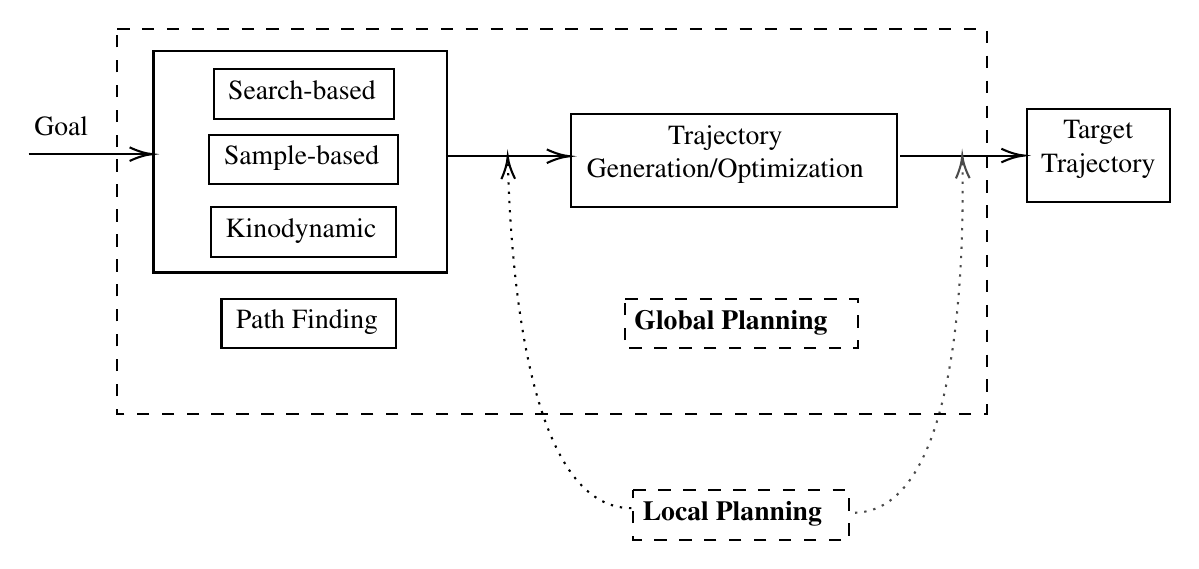
\begin{tikzpicture}[x=0.75pt,y=0.75pt,yscale=-1,xscale=1]
%uncomment if require: \path (0,267); %set diagram left start at 0, and has height of 267

%Shape: Rectangle [id:dp575866165243341] 
\draw   (89.56,19.67) -- (230.89,19.67) -- (230.89,126.44) -- (89.56,126.44) -- cycle ;
%Straight Lines [id:da8414235785777104] 
\draw    (230.44,70.44) -- (288,70.44) ;
\draw [shift={(290,70.44)}, rotate = 180] [color={rgb, 255:red, 0; green, 0; blue, 0 }  ][line width=0.75]    (10.93,-3.29) .. controls (6.95,-1.4) and (3.31,-0.3) .. (0,0) .. controls (3.31,0.3) and (6.95,1.4) .. (10.93,3.29)   ;
%Straight Lines [id:da08815651015896142] 
\draw    (29.44,69.44) -- (87,69.44) ;
\draw [shift={(89,69.44)}, rotate = 180] [color={rgb, 255:red, 0; green, 0; blue, 0 }  ][line width=0.75]    (10.93,-3.29) .. controls (6.95,-1.4) and (3.31,-0.3) .. (0,0) .. controls (3.31,0.3) and (6.95,1.4) .. (10.93,3.29)   ;
%Straight Lines [id:da22108099082080424] 
\draw    (449.44,70.11) -- (507,70.11) ;
\draw [shift={(509,70.11)}, rotate = 180] [color={rgb, 255:red, 0; green, 0; blue, 0 }  ][line width=0.75]    (10.93,-3.29) .. controls (6.95,-1.4) and (3.31,-0.3) .. (0,0) .. controls (3.31,0.3) and (6.95,1.4) .. (10.93,3.29)   ;
%Curve Lines [id:da017803972324741846] 
\draw [color={rgb, 255:red, 0; green, 0; blue, 0 }  ,draw opacity=1 ] [dash pattern={on 0.84pt off 2.51pt}]  (319.78,240) .. controls (270.94,240) and (261.74,130.66) .. (260.26,72.2) ;
\draw [shift={(260.22,70.44)}, rotate = 88.68] [color={rgb, 255:red, 0; green, 0; blue, 0 }  ,draw opacity=1 ][line width=0.75]    (10.93,-3.29) .. controls (6.95,-1.4) and (3.31,-0.3) .. (0,0) .. controls (3.31,0.3) and (6.95,1.4) .. (10.93,3.29)   ;
%Curve Lines [id:da912860022154641] 
\draw [color={rgb, 255:red, 74; green, 74; blue, 74 }  ,draw opacity=1 ] [dash pattern={on 0.84pt off 2.51pt}]  (427.56,242.22) .. controls (475.74,240.9) and (480.46,130.36) .. (479.26,71.87) ;
\draw [shift={(479.22,70.11)}, rotate = 88.68] [color={rgb, 255:red, 74; green, 74; blue, 74 }  ,draw opacity=1 ][line width=0.75]    (10.93,-3.29) .. controls (6.95,-1.4) and (3.31,-0.3) .. (0,0) .. controls (3.31,0.3) and (6.95,1.4) .. (10.93,3.29)   ;
%Shape: Rectangle [id:dp5818665047698117] 
\draw  [dash pattern={on 4.5pt off 4.5pt}] (72,9) -- (491,9) -- (491,194.5) -- (72,194.5) -- cycle ;

% Text Node
\draw    (122.33,139) -- (206.33,139) -- (206.33,163) -- (122.33,163) -- cycle  ;
\draw (125.33,143) node [anchor=north west][inner sep=0.75pt]   [align=left] {\begin{minipage}[lt]{55.15pt}\setlength\topsep{0pt}
\begin{center}
{\fontfamily{ptm}\selectfont Path Finding}
\end{center}

\end{minipage}};
% Text Node
\draw    (118.5,28.5) -- (205.5,28.5) -- (205.5,52.5) -- (118.5,52.5) -- cycle  ;
\draw (121.5,32.5) node [anchor=north west][inner sep=0.75pt]   [align=left] {\begin{minipage}[lt]{57.1pt}\setlength\topsep{0pt}
\begin{center}
{\fontfamily{ptm}\selectfont Search-based}
\end{center}

\end{minipage}};
% Text Node
\draw    (116.5,60) -- (207.5,60) -- (207.5,84) -- (116.5,84) -- cycle  ;
\draw (119.5,64) node [anchor=north west][inner sep=0.75pt]   [align=left] {\begin{minipage}[lt]{59.94pt}\setlength\topsep{0pt}
\begin{center}
{\fontfamily{ptm}\selectfont Sample-based}
\end{center}

\end{minipage}};
% Text Node
\draw    (117.33,95) -- (206.33,95) -- (206.33,119) -- (117.33,119) -- cycle  ;
\draw (120.33,99) node [anchor=north west][inner sep=0.75pt]   [align=left] {\begin{minipage}[lt]{58.25pt}\setlength\topsep{0pt}
\begin{center}
{\fontfamily{ptm}\selectfont Kinodynamic}
\end{center}

\end{minipage}};
% Text Node
\draw    (290.78,50) -- (447.78,50) -- (447.78,95) -- (290.78,95) -- cycle  ;
\draw (293.78,54) node [anchor=north west][inner sep=0.75pt]   [align=left] {\begin{minipage}[lt]{104.69pt}\setlength\topsep{0pt}
\begin{center}
{\fontfamily{ptm}\selectfont Trajectory }\\{\fontfamily{ptm}\selectfont Generation/Optimization}
\end{center}

\end{minipage}};
% Text Node
\draw (30.67,49.67) node [anchor=north west][inner sep=0.75pt]   [align=left] {{\fontfamily{ptm}\selectfont Goal}};
% Text Node
\draw    (510.33,47.67) -- (579.33,47.67) -- (579.33,92.67) -- (510.33,92.67) -- cycle  ;
\draw (513.33,51.67) node [anchor=north west][inner sep=0.75pt]   [align=left] {\begin{minipage}[lt]{44.84pt}\setlength\topsep{0pt}
\begin{center}
{\fontfamily{ptm}\selectfont Target }\\{\fontfamily{ptm}\selectfont Trajectory}
\end{center}

\end{minipage}};
% Text Node
\draw  [dash pattern={on 4.5pt off 4.5pt}]  (320.8,231.22) -- (424.8,231.22) -- (424.8,255.22) -- (320.8,255.22) -- cycle  ;
\draw (323.8,235.22) node [anchor=north west][inner sep=0.75pt]   [align=left] {{\fontfamily{ptm}\selectfont \textbf{Local Planning}}};
% Text Node
\draw  [dash pattern={on 4.5pt off 4.5pt}]  (316.8,139) -- (428.8,139) -- (428.8,163) -- (316.8,163) -- cycle  ;
\draw (319.8,143) node [anchor=north west][inner sep=0.75pt]   [align=left] {{\fontfamily{ptm}\selectfont \textbf{Global Planning}}};


\end{tikzpicture}
\end{adjustbox}
\caption{Hierarchical planning pipeline: The path-finding module 
finds a geometric collision-free path, and then trajectory
optimization module generates a state-admissable kinodynamic
feasibility trajectory. Local planning methods can be 
incorporated in different stages.}
\label{fig:concept}
\end{figure}
